%
\hsection{Installing yEd on Microsoft Windows}%
%
\begin{figure}%
\centering%
%
\subfloat[][%
We will download \yEd\ from the website \url{https://www.yworks.com/products/yed}. %
We surf to this website and scroll down.%
\label{fig:installingYedWindows01website}%
]{\tightbox{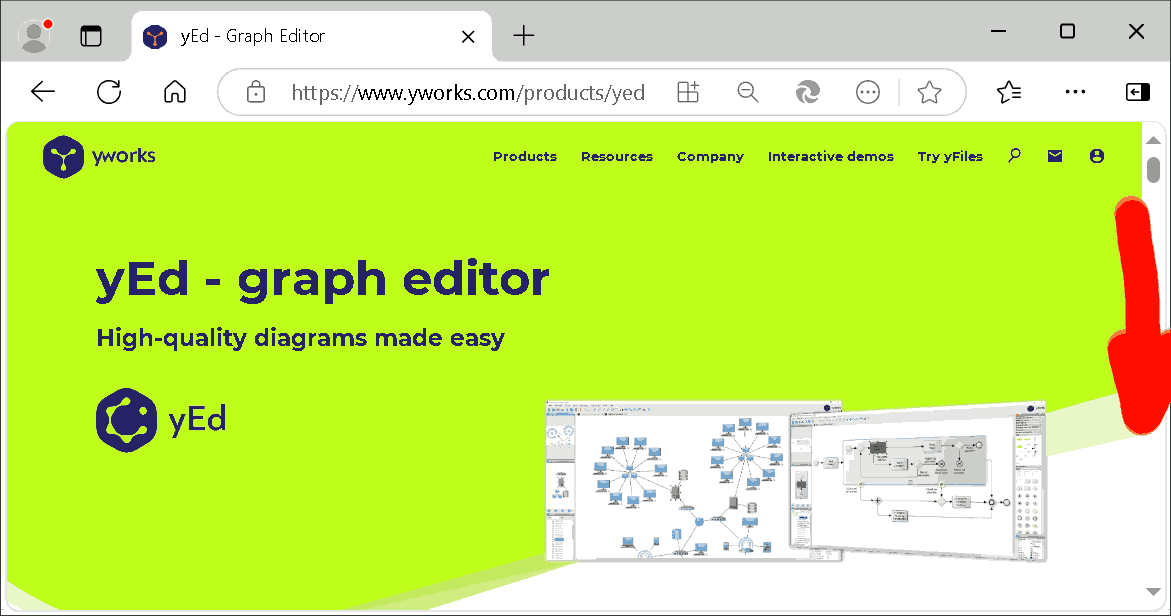
\includegraphics[width=0.48\linewidth]{\currentDir/installingYedWindows01website}}}%
%
\floatSep%
%
\subfloat[][%
We locate the \menu{Download} button and click on it.%
\label{fig:installingYedWindows02download}%
]{\tightbox{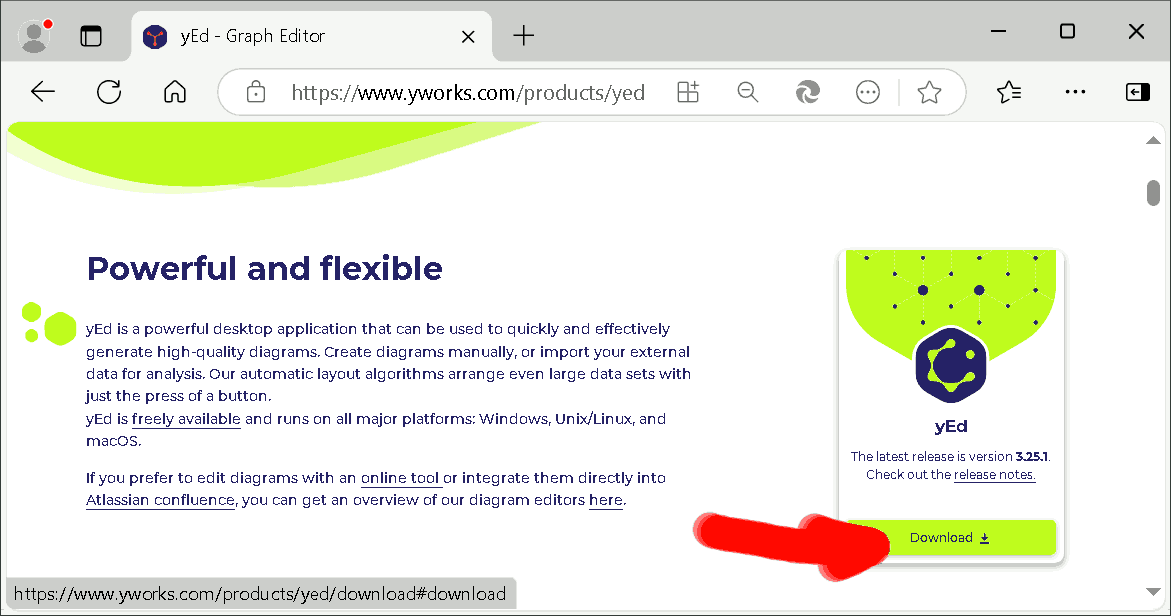
\includegraphics[width=0.48\linewidth]{\currentDir/installingYedWindows02download}}}%
%
\floatRowSep%
%
\subfloat[][%
We click on \menu{yEd for Windows}.%
\label{fig:installingYedWindows03downloadForWindows}%
]{\tightbox{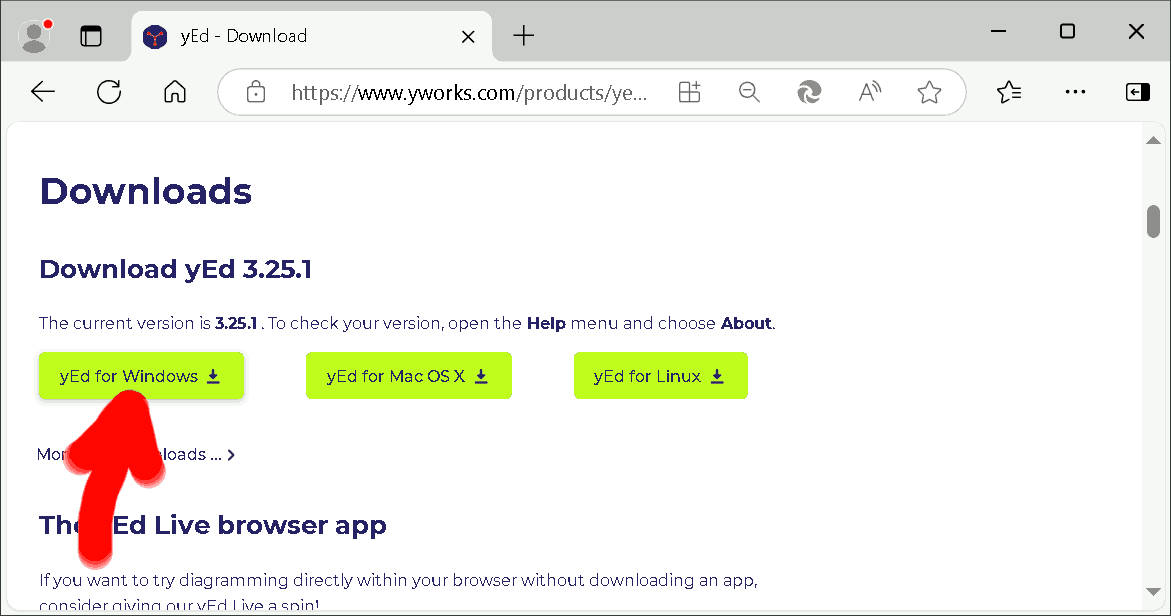
\includegraphics[width=0.48\linewidth]{\currentDir/installingYedWindows03downloadForWindows}}}%
%
\floatSep%
%
\subfloat[][%
In order to download the program, we have to accept the license agreement. %
Then we can click on \menu{Download}.%
\label{fig:installingYedWindows05acceptLicenseAndDownload}%
]{\tightbox{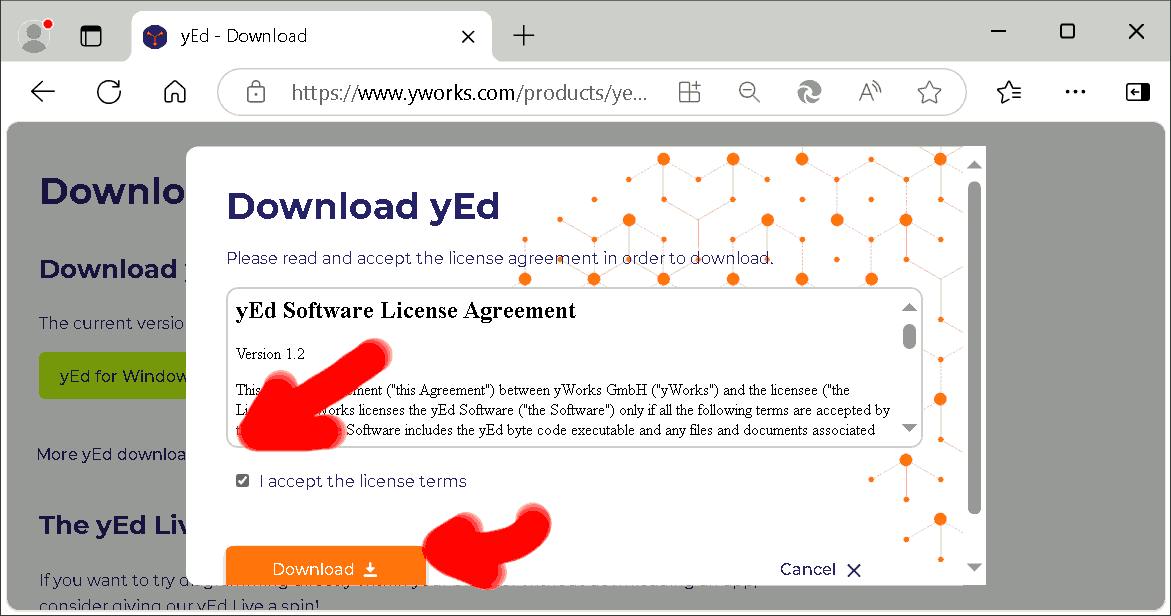
\includegraphics[width=0.48\linewidth]{\currentDir/installingYedWindows05acceptLicenseAndDownload}}}%
%
\floatRowSep%
%
\subfloat[][%
Once the download completes, we click \menu{Open file} or the equivalent option in your browser.%
\label{fig:installingYedWindows07downloaded}%
]{\tightbox{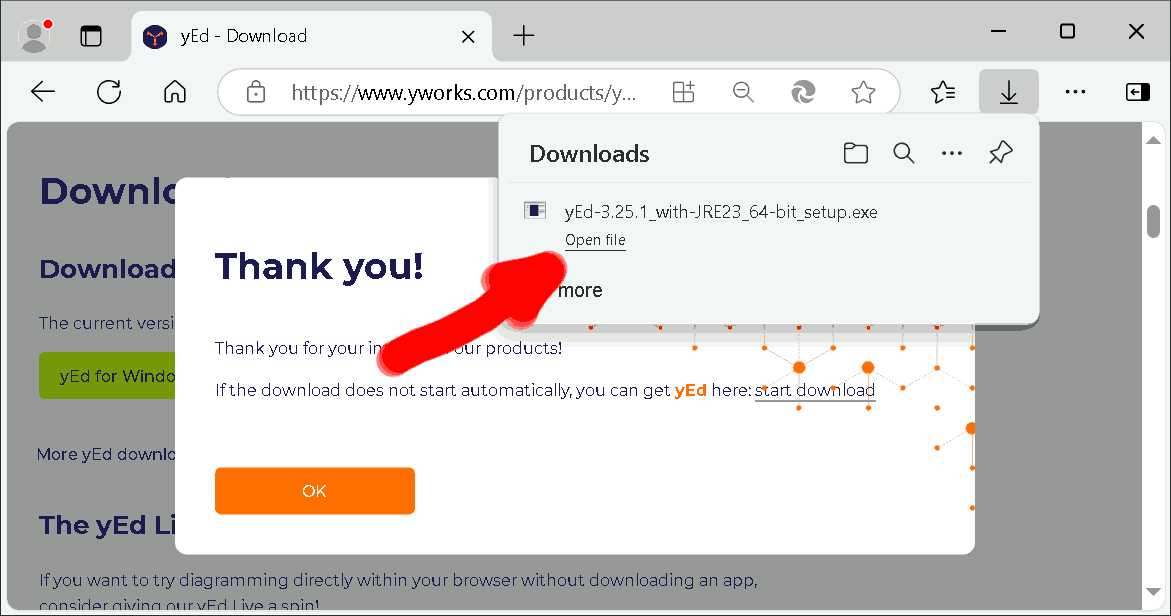
\includegraphics[width=0.48\linewidth]{\currentDir/installingYedWindows07downloaded}}}%
%
\floatSep%
%
\subfloat[][%
The installation wizard begins the setup.%
\label{fig:installingYedWindows08preparingInstall}%
]{\tightbox{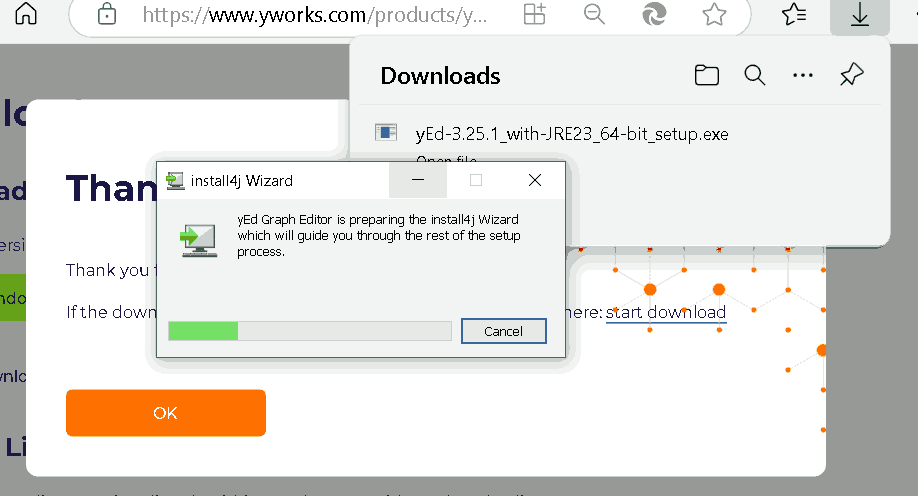
\includegraphics[width=0.48\linewidth]{\currentDir/installingYedWindows08preparingInstall}}}%
%
\caption{Installing \yEd\ under \microsoftWindows.}%
\label{fig:installingYedWindows:A}%
\end{figure}%
%
\begin{figure}%
\ContinuedFloat%
\centering%
%
\subfloat[][%
\microsoftWindows\ asks us whether we want to permit the program to make changes on your computer~(=~install something). %
We click~\menu{Yes}.%
\label{fig:installingYedWindows09shouldWeInstall}%
]{\tightbox{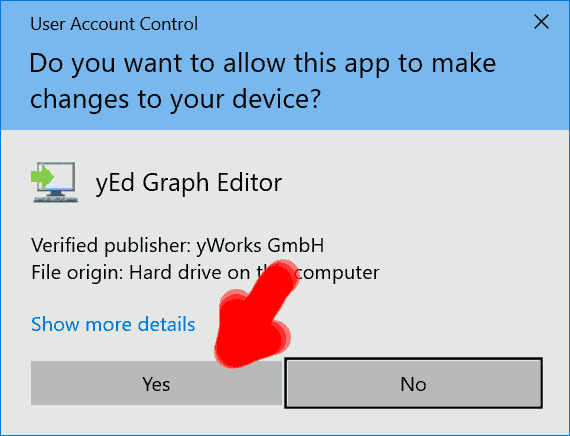
\includegraphics[width=0.48\linewidth]{\currentDir/installingYedWindows09shouldWeInstall}}}%
%
\floatSep%
%
\subfloat[][%
We click \menu{Next} in the installer's welcome screen.%
\label{fig:installingYedWindows10welcome}%
]{\tightbox{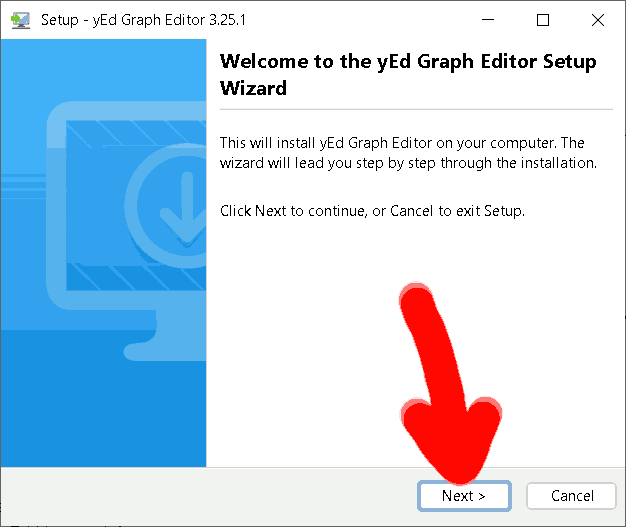
\includegraphics[width=0.48\linewidth]{\currentDir/installingYedWindows10welcome}}}%
%
\floatRowSep%
%
\subfloat[][%
In order to install \yEd, we must agree to the license agreement. %
If you are OK with it, accept the agreement and click~\menu{Next}.%
\label{fig:installingYedWindows12licenseAccept}%
]{\tightbox{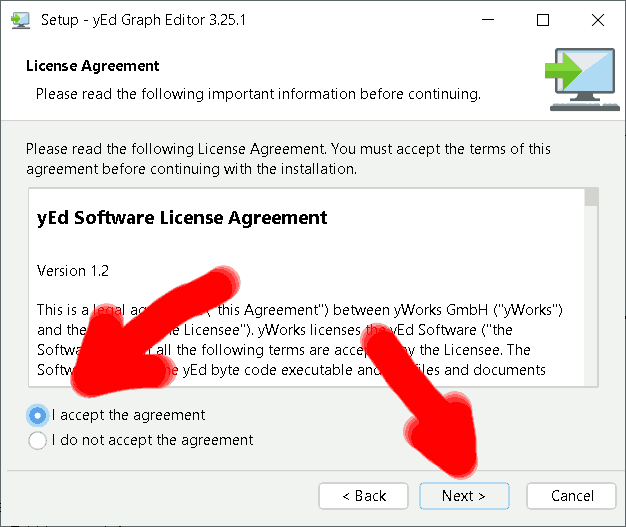
\includegraphics[width=0.48\linewidth]{\currentDir/installingYedWindows12licenseAccept}}}%
%
\floatSep%
%
\subfloat[][%
We do not change the installation destination and click~\menu{Next}.%
\label{fig:installingYedWindows13destination}%
]{\tightbox{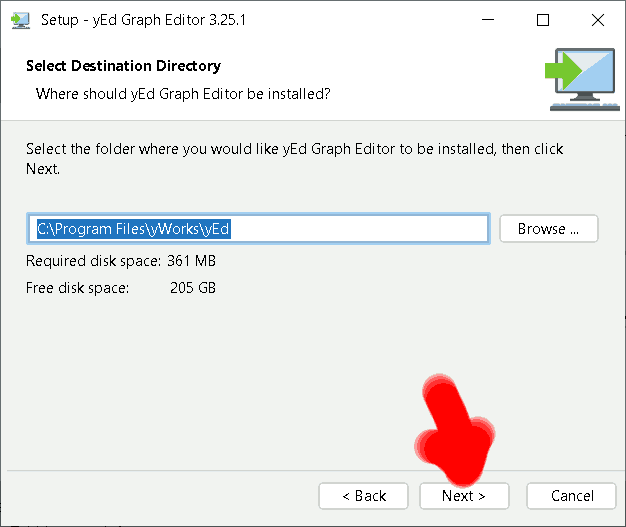
\includegraphics[width=0.48\linewidth]{\currentDir/installingYedWindows13destination}}}%
%
\floatRowSep%
%
\subfloat[][%
We do not change the start menu settings and click~\menu{Next}.%
\label{fig:installingYedWindows14startMenu}%
]{\tightbox{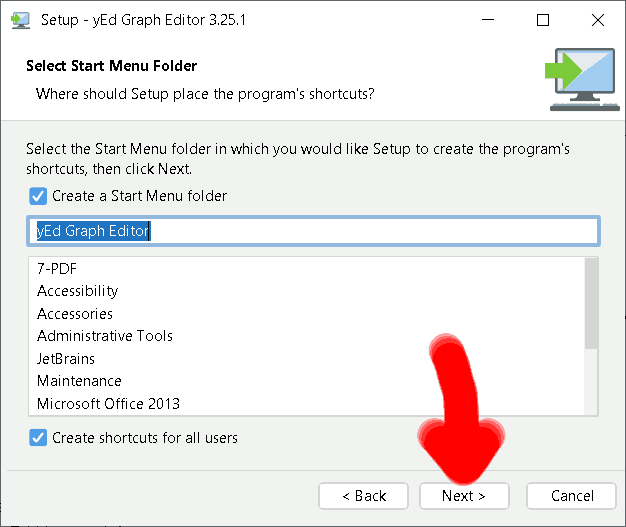
\includegraphics[width=0.48\linewidth]{\currentDir/installingYedWindows14startMenu}}}%
%
\floatSep%
%
\subfloat[][%
We do not change the file type associations and click~\menu{Next}.%
\label{fig:installingYedWindows15fileSuffixes}%
]{\tightbox{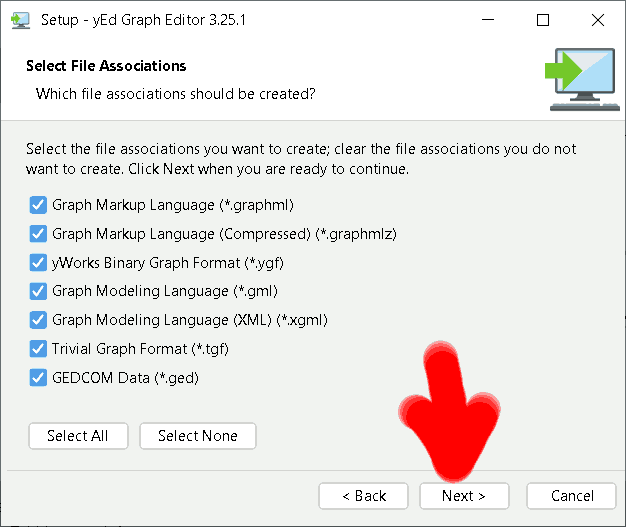
\includegraphics[width=0.48\linewidth]{\currentDir/installingYedWindows15fileSuffixes}}}%
%
\caption{Installing \yEd\ under \microsoftWindows~(continued).}%
\label{fig:installingYedWindows:B}%
\end{figure}%
%
\begin{figure}%
\ContinuedFloat%
\centering%
%
\subfloat[][%
We do not change the additional task settings and click~\menu{Next}.%
\label{fig:installingYedWindows17icon}%
]{\tightbox{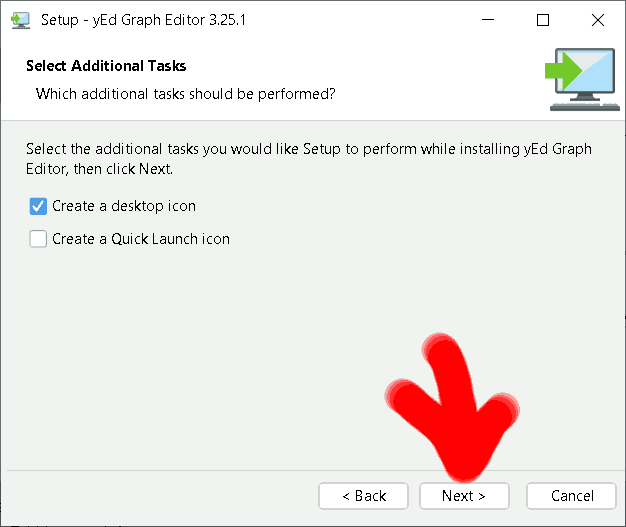
\includegraphics[width=0.48\linewidth]{\currentDir/installingYedWindows17icon}}}%
%
\floatSep%
%
\subfloat[][%
The installation begins.%
\label{fig:installingYedWindows18installing}%
]{\tightbox{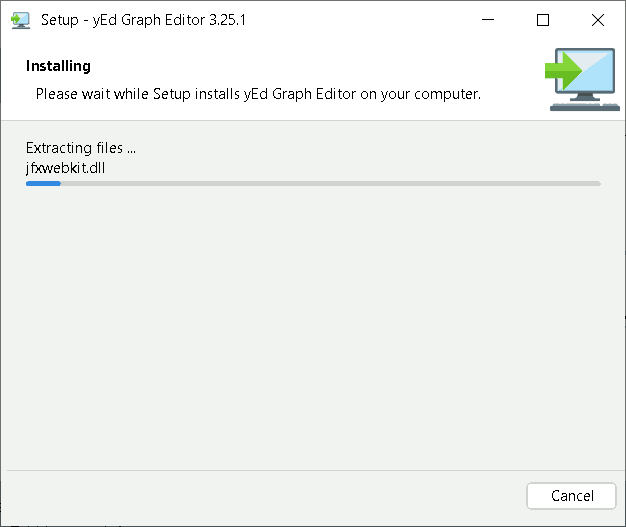
\includegraphics[width=0.48\linewidth]{\currentDir/installingYedWindows18installing}}}%
%
\floatRowSep%
%
\subfloat[][%
The installation completes. %
We mark \inQuotes{Run yEd Graph Editor} and click on~\menu{Finish}.%
\label{fig:installingYedWindows19doneRun}%
]{\tightbox{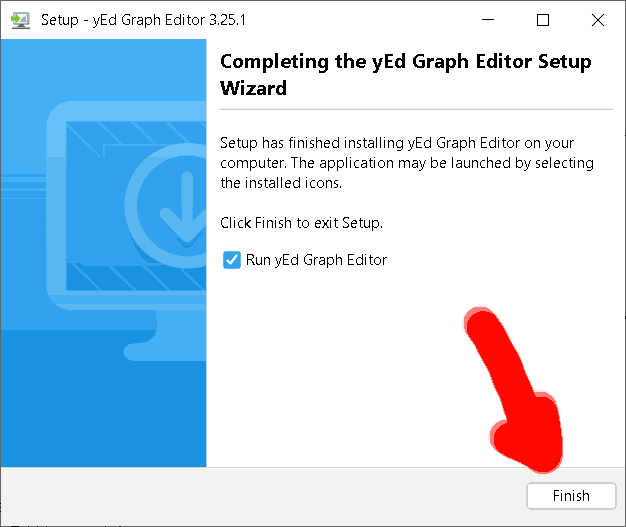
\includegraphics[width=0.48\linewidth]{\currentDir/installingYedWindows19doneRun}}}%
%
\floatSep%
%
\subfloat[][%
The \yEd\ spash screen appears.%
\label{fig:installingYedWindows20splash}%
]{\tightbox{
\includegraphics[width=0.48\linewidth]{\currentDir/installingYedWindows20splash}}}%
%
\floatRowSep%
%
\subfloat[][%
\yEd\ is installed and running.%
\label{fig:installingYedWindows21running}%
]{\tightbox{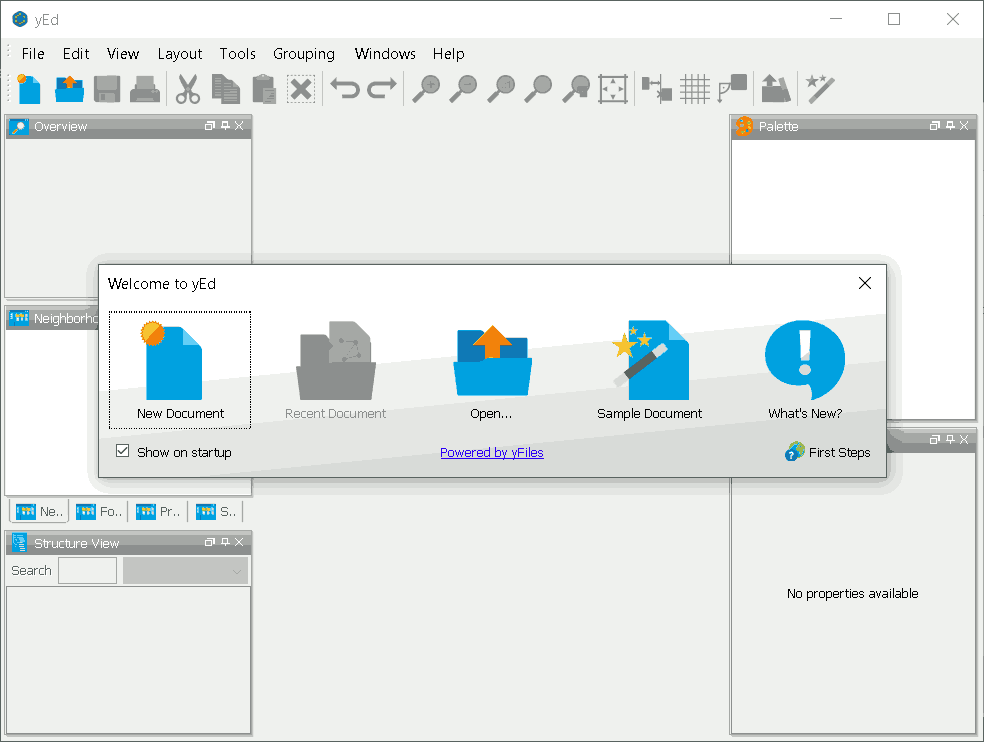
\includegraphics[width=0.6\linewidth]{\currentDir/installingYedWindows21running}}}%
%
\caption{Installing \yEd\ under \microsoftWindows~(continued).}%
\label{fig:installingYedWindows:C}%
\end{figure}%
%
Installing \yEd\ under \microsoftWindows\ is very easy.
We basically just have to download and run the installer.
We will download \yEd\ from the website \url{https://www.yworks.com/products/yed}.
We surf to this website in \cref{fig:installingYedWindows01website} and then need to scroll down.
We locate the \menu{Download} button on the website and click on it in \cref{fig:installingYedWindows02download}.

On the next page, we get to choose for which \pgls{OS} we want to install \yEd.
We click on \menu{yEd for Windows} in \cref{fig:installingYedWindows03downloadForWindows}.
In order to download the program, we have to accept the license agreement.
We carefully read the agreement.
If we agree to it, we can tick the corresponding box and then we can click on \menu{Download} in \cref{fig:installingYedWindows05acceptLicenseAndDownload}.

Once the download completes, we click \menu{Open file} or the equivalent option in your browser in \cref{fig:installingYedWindows07downloaded}.
The installation wizard begins the setup in \cref{fig:installingYedWindows08preparingInstall}.
Shortly thereafter, \microsoftWindows\ asks us whether we want to permit the program to make changes on your computer, i.e., to install \yEd.
We click~\menu{Yes} in \cref{fig:installingYedWindows09shouldWeInstall}.

The installer's welcome screen appears.
We click \menu{Next} in \cref{fig:installingYedWindows10welcome}.
In order to install \yEd, we must agree to the license agreement.
If you are OK with it, accept the agreement, tick the corresponding box, and click~\menu{Next}, as shown in \cref{fig:installingYedWindows12licenseAccept}.

Then we can choose where to install \yEd.
We do not change the installation destination and click~\menu{Next} in \cref{fig:installingYedWindows13destination}.
The option whether and where we want to add buttons to the start menu if \microsoftWindows\ appears.
We do not change the start menu settings and click~\menu{Next} in \cref{fig:installingYedWindows14startMenu}.
The installer asks which files should be associated with \yEd.
We do not change the file type associations and click~\menu{Next} in \cref{fig:installingYedWindows15fileSuffixes}.
In the screen for additional tasks, we could decide not to add a desktop icon, for instance.
However, in \cref{fig:installingYedWindows17icon}, we do not change the additional task settings and click~\menu{Next}.
The installation begins in \cref{fig:installingYedWindows18installing}.

Soon thereafter, the installation completes.
In the final screen shown in \cref{fig:installingYedWindows19doneRun}, we make sure that \inQuotes{Run yEd Graph Editor} is marked and click on~\menu{Finish}.

Now, the \yEd\ spash screen appears in \cref{fig:installingYedWindows20splash}.
\yEd\ is installed and running and we can begin to use it, as illustrated in \cref{fig:installingYedWindows21running}.%
%
\FloatBarrier%
\endhsection%
%
